\documentclass[10pt,twocolumn]{extarticle}

\usepackage[margin=0.55in,columnsep=0.22in]{geometry}
\usepackage[T1]{fontenc}
\usepackage{lmodern}
\usepackage{microtype}
\usepackage{amsmath,amssymb}
\usepackage{booktabs}
\usepackage{tabularx}
\usepackage{array}
\usepackage{graphicx}
\usepackage{tikz}
\usetikzlibrary{arrows.meta,positioning,fit}
\usepackage{xcolor}
\usepackage{enumitem}
\usepackage[font=footnotesize,labelfont=bf]{caption}
\usepackage{titlesec}
\usepackage[most]{tcolorbox}
\usepackage{hyperref}
\usepackage{flushend}

\hypersetup{colorlinks=true,linkcolor=blue!40!black,citecolor=blue!40!black,
  urlcolor=blue!50!black,
  pdftitle={What a Frozen Detector Representation Resolves: Measurement
            Geometry, Training Support, and Consequence-Aware Diagnosis},
  pdfauthor={Dowling Wong}}
\setlength{\parindent}{0pt}
\setlength{\parskip}{1.0pt}
\setlist{nosep,leftmargin=*,topsep=1pt}
\titlespacing*{\section}{0pt}{3.5pt}{1pt}
\titleformat{\section}{\small\bfseries}{\thesection}{0.4em}{}
\newcolumntype{Y}{>{\raggedright\arraybackslash}X}

\title{\vspace{-1.55em}\textbf{What a Frozen Detector Representation Resolves:\\[-0.18em]
Measurement Geometry, Training Support, and Consequence-Aware Diagnosis}\\[-0.12em]
\normalsize Collaboration concept note (formerly \emph{Consequence-aware failure diagnostics for learned particle-reconstruction representations})}
\author{Dowling Wong}
\date{16 September 2026 (two-claim revision)}

\begin{document}
\maketitle
\vspace{-1.9em}

\begin{abstract}
A frozen reconstruction model deployed on a physics detector carries a
contract: an assumed noise covariance and a training distribution. When either
moves, a monitor must say which declared mechanism moved and whether the
physics result is harmed. This note proposes a study that makes exactly two
claims and tests both against a strong, committed generic monitor with
identical alarm-time information. \emph{Claim 1:} on declared,
alarm-time-observable interventions, statistics of a model's intermediate
representations add acquisition-versus-valid-physics attribution information
beyond a generic arm that already holds input quality, outputs, uncertainty,
the final embedding, noise-only quality statistics and the same
reference-distance transforms --- measured as a paired macro-F1 difference on
a hard, signature-matched evaluation set with capacity-matched and hook-drop
controls, and with abstention on undeclared families evaluated empirically.
\emph{Claim 2:} a predeclared task-sensitive representation score, the length
of a window's deviation in the metric $J_y^{\top}W_yJ_y$ pulled back from
declared physics outputs, ranks scientific harm on held-out physical
intervention cells better than the committed generic score --- measured as a
paired AUROC difference for $K\ge\kappa_m$ with the cell as the resampling
unit. The measurement metric $\tilde J_g^{\top}\tilde J_g$ (the Gaussian
Fisher information under the assumed covariance) and the task metric are kept
apart; resolvability is not read as training support, which is estimated and
validated separately; acquisition and support signatures are stated as
conditional hypotheses that the development table already partly contradicts.
The evidence ladder is deliberately short: a controlled waveform simulator in
which the assumed and realized covariance are both known, run on a trained
nonlinear subject, plus one independent transfer arm selected by readiness and
licence gates; TIDMAD is an external check if its physical endpoint is
defensible. A negative result --- intermediate hooks do not justify their
cost --- is reportable if the positive controls, precision and baseline
design pass. No result in this note is claimed; the protocol prototype, its
tests and a non-citable development smoke exist, and no protocol is frozen.
\end{abstract}

\section{Gap and contribution}

\textbf{The question.} Cross-detector pre-training has shown that one
sensor-level recipe learns useful representations on three physically
different detectors, that those representations cut supervision by orders of
magnitude, and that linear probes find physics in them~\cite{panda2}. That
answers how general a \emph{recipe} can be. It does not say why a
representation takes the form it does, or when it stops resolving the physics
it was trained on. The companion theory~\cite{paper1} gives the determinants
for a calibrated readout: the measurement fixes the metric $\Sigma^{-1}$, the
architecture fixes the admissible class, and the training data fix the
excited latent support; the wrong metric learns the wrong physical structure
on planted data. This study asks the deployment half of the same question on
frozen models: \emph{which determinant moved, is the physics still resolved,
and does it matter} --- with the determinants supplying the predictions rather
than a list of failure modes.

Existing shift monitors can detect changes in inputs, outputs, or embeddings,
but a scientific reconstruction pipeline requires two additional distinctions:
whether the change reflects corrupted acquisition or valid but under-supported
physics, and whether the detected change materially degrades a physics result.
We test whether intermediate representations improve this attribution beyond
generic monitoring at the same false-alert budget, while allowing abstention on
ambiguous or unseen failures. The attribution claim is conditional on the
declared simulator and forward model: unknown physics and model
misspecification are not identifiable from a response profile alone and are
routed to abstention.

No public dataset can decide these questions. None carries a known
assumed-versus-realized covariance --- simulation tools that \emph{synthesise}
correlated multichannel noise from a specified spectrum are open and recent
(\cite{pytessim}; Wire-Cell's per-band colorer
matrices~\cite{wirecell}, on the measured coherent-noise model
of~\cite{microboone2017noise}), but none reports the realized covariance of the
ensemble it drew, which is what makes $\kappa(\hat\Sigma^{-1}\Sigma)$ a measured
lever rather than a nominal setting --- and none is event-paired across the factors
a causal claim must vary: the released NuBench sets are independent
per-geometry productions, and TIDMAD's own authors disclaim the scientific
meaning of its denoising score. The study therefore produces its own evidence
in two designed datasets --- a controlled-covariance waveform set
(\textbf{ORACLE-Cov}) and a paired multi-geometry point-cloud set
(\textbf{ORACLE-Paired}), the latter a citable artifact in its own right ---
and uses TIDMAD as the real-data check. The tiers are ordered: predictions
fixed on the mechanism tier are pre-registered before the single confirmatory
run on the realism tier.

In waveform reconstruction, structured acquisition noise induces a likelihood
geometry through the inverse covariance: the correct residual weighting is
$\Sigma^{-1}$, and a model evaluated under the wrong weighting can prefer
reconstructions that are worse in the metric the instrument implies.
Architecture and training coverage further determine which physically relevant
distinctions survive into the representation~\cite{paper1}. This study asks
whether violations of these assumptions can be diagnosed after training, and
whether a detected violation is scientifically consequential. The question has
become concrete: cross-modality frozen backbones now exist --- Panda~V2 is
pre-trained with one recipe on LArTPC, collider-TPC and water-Cherenkov data
and adapted with $10^3$ labels per detector~\cite{panda2} --- and their authors
list transfer across detectors and from simulation to real data as untested.
Those are exactly the acquisition-shift and support-shift questions posed
here, on a frozen public model. The artifact is a
reproducible experiment suite---configurations, adapters, hooks, replay
scripts, and reports---not a maintained software product.

\textbf{Contribution, and what would refute it.} Relative to the shift
literature the study adds a setting and two paired tests, not a monitor.
Failing Loudly~\cite{rabanser2019} established that two-sample tests on a
pre-trained classifier's representation detect shift well and that a domain
classifier characterizes it; shift malignancy there is classification
accuracy. Zhang et al.~\cite{zhang2023} attribute a performance change to
shifted mechanisms with labelled target data. Unlabelled performance
estimation~\cite{guillory2021,garg2022} predicts a classifier's aggregate
target accuracy from confidences under stated assumptions on the shift.
Conformal methods~\cite{angelopoulos2021} give marginal coverage under
exchangeability and no guarantee against arbitrary unknown shifts. What this
study can establish beyond these is narrow and checkable: on a frozen physics
reconstruction model under declared interventions with a known assumed
covariance, (i)~whether strictly internal representation statistics add
attribution information beyond a generic arm holding the same alarm-time
side information and the same distance transforms (Claim~1), and
(ii)~whether a task-sensitive representation score orders held-out
intervention cells by a physics loss against evaluation-only truth better
than a committed generic score, including harm that arrives without a strong
alarm (Claim~2). Claim~1 is refuted by equivalence or detriment on the hard
contrasts, or by a gain the ablations assign to input/output transformations,
noise-only records, feature count or event identity; Claim~2 by a paired
interval that includes zero without meeting the equivalence rule, by
systematic low-alarm/high-harm failures, or by a gain that vanishes on
held-out physical families. We do not claim a first or an exhaustive search;
the components are established and cited as such.

\textbf{Position relative to learned-geometry reconstruction.} The subjects
of this study are models that \emph{learn} the geometry of the measurement:
distance-weighted graph networks that place every sensor in a learned
coordinate space~\cite{gravnet}, potential-based objectives that attach to
each vertex a learned weight for whether it can represent its
object~\cite{objcond}, and cross-detector pre-training
recipes~\cite{panda2}. None of these carries a statement of what its
representation can resolve once the acquisition or the physics moves; recent
benchmarks of physics foundation models report regime-dependent scores across
distribution shifts without a mechanism~\cite{fmbench}. The learned
resolvability weight of object condensation is the closest relative of the
resolvability diagnostic of Section~\ref{sec:mechanism} (the rank of
$M_{\mathrm{recon}}$), which computes a related quantity for a \emph{frozen}
model from its reconstruction Jacobian and the assumed covariance, with no
training signal. Nothing here proposes a new reconstruction architecture; the
contribution is the two paired tests and the designed data on which they can
fail.

\textbf{Identifiability limit.} Diagonalizing a covariance yields decorrelated
statistical modes, not labeled physical sources: $\Sigma=\Sigma_1+\Sigma_2$
admits infinitely many positive-semidefinite splits, and low-rank factors are
rotation-degenerate. All attribution here is over \emph{declared intervention
families} under a stated simulator. Observing a response profile does not
identify the cause of an unknown real shift, and we make no such claim.

\section{Failure contracts}

Three declared labels, frozen before evaluation.

\textbf{N---acquisition-contract violation.} For this study the closed family
is power-spectral-density (PSD) or covariance change, jitter, drift, spectral
lines, glitches, tails, hit thinning, and channel or module loss. The
measurement violates a declared acquisition condition; no broader N claim is
made.

\textbf{S---training-support shift.} Window or event composition moves toward
physical strata that are sparse under the clean training distribution. The
events themselves are clean and physically valid; only the support has moved.

\textbf{E---evaluation-contract fault.} Wrong units, coordinate ordering,
output semantics, PSD convention, or metric implementation. This is a pipeline
bug, not a distribution shift.

\textbf{N versus S is the scientific core.} E is decided by deterministic
schema and range invariants, so it is reported as a gate result, not as a class
in a classification score. The informative and difficult separation is N from
S. N and S may both move the observed input distribution, so generic
input-shift detection alone cannot distinguish them. Evidence for N comes from
acquisition-quality indicators, paired corruption interventions, or known
violations of the measurement model. S is defined by physically valid,
uncorrupted events that occupy low-density regions of the clean training
support. The scientific problem is therefore not whether the input changed, but
whether the change reflects corrupted measurement or valid but under-supported
physics. Section~\ref{sec:mechanism} states why the two leave different
geometric signatures in a frozen representation, which is what makes N versus
S a prediction rather than a label. That distinction is what matters operationally: discarding S rejects
physically valid events, whereas rejecting N removes measurements that violate
the declared acquisition contract.

\section{Two metrics, and what a frozen representation can resolve}
\label{sec:mechanism}

Write the declared forward model as $x=g(r)+n$, $n\sim\mathcal N(0,\Sigma)$,
where $x\in\mathbb R^{CN}$ is the sampled measurement, $r\in\mathbb R^{d}$ the
representation being monitored (for the analytic subject, the pooled latent
$z$; for a network, any hooked stage), $g$ the reconstruction back into
measurement space and $y=h(r)\in\mathbb R^{t}$ the map to the declared physics
outputs (amplitude, arrival time, shape). Two pullback metrics live on $r$, and
they are different objects.

\textbf{Measurement metric.} Under the assumed covariance $\hat\Sigma$ the
Fisher information of $r$ is $I(r)=J_g^{\top}\hat\Sigma^{-1}J_g$ with
$J_g=\partial g/\partial r$ --- the standard Gaussian-model
result~\cite{kay1993}; in whitened coordinates
$\tilde J_g=\hat\Sigma^{-1/2}J_g$ it is $M_{\mathrm{recon}}=\tilde
J_g^{\top}\tilde J_g$, unit-free (whitened residual per sample), local to the
reference point, and dependent on the \emph{assumed} covariance --- the
operational one --- never the realized $\Sigma$. Its eigen-directions above a
rank threshold are the directions the measurement \emph{resolves}; those below
are weakly resolved and, where $\operatorname{rank}M_{\mathrm{recon}}<d$, not
locally identifiable at all. That is a local identifiability statement. It is
not a statement about which directions the training distribution excited, and
this paper no longer reads it as one.

\textbf{Task metric.} With $J_y=\partial y/\partial r$ and a declared
positive semi-definite weight $W_y$ in physics-output units (a diagonal of
inverse squared resolution requirements, or a one-hot selecting the
consequence target), $M_{\mathrm{task}}=J_y^{\top}W_yJ_y$ measures how far a
representation displacement moves the declared outputs. $\Sigma$ does not
enter: $J_y$ maps to outputs, not to measurements, so an expression of the
form $J_y^{\top}\Sigma^{-1}J_y$ is dimensionally invalid and is not used.
The task-sensitive score of Claim~2 is the length
$\|r-\bar r\|_{M_{\mathrm{task}}}$ of a window's deviation from the reference
mean, standardized on clean windows. Neither metric measures realized
scientific harm; Claim~2 tests that connection empirically.

\textbf{Training support is estimated, not inferred from rank.} Whether a
window lies where the training distribution placed mass is estimated by a
separate score on the reference representation --- a shrinkage Mahalanobis
distance combined with a $k$-nearest-neighbour distance, each standardized by
its clean reference quantile --- validated before use on constructed
in-support and out-of-support controls, and used only when that control
passes a declared floor. Valid rare physics can therefore be
\emph{in-support-but-rare} or \emph{outside estimated support}; the
development table already contains both kinds (Section~\ref{sec:testbeds}).

\textbf{Conditional signatures, not a dichotomy.} The earlier reading that
acquisition shift stays in the excited span while support shift lives in its
complement is contradicted by the development table: gain drift, channel loss
and timing jitter --- acquisition changes by contract --- produce
representation shifts with out-of-span fractions near one, and in-span rare
physics moves the representation a great deal while leaving every
noise-only statistic at its reference. The mechanism section therefore states
conditional signatures, each a hypothesis the attribution arms test:
(i)~a covariance-only acquisition change ($\hat\Sigma\neq\Sigma$, $g$
unchanged) changes noise-only residual statistics --- whitened variance,
residual spectrum, residual channel correlation on random-trigger records ---
without a consistent representation mean shift; (ii)~a structural acquisition
change (gain, channel loss, jitter) can produce both a representation shift
and a residual shift; (iii)~valid rare physics leaves the noise-only
statistics at their reference and moves the representation either inside the
resolved span (head-limited) or outside estimated support; (iv)~origin and
harm are separate axes. The signatures do not prove causal origin outside the
declared intervention design; the classifier of Claim~1 tests whether their
collection, computed from intermediate hooks, adds information beyond the
generic arm that already sees (i)--(iii) at the input, output and final
embedding.

\textbf{Invariance, stated exactly.} Every reported statistic is labelled with
the group under which it is invariant. Reference Mahalanobis distances with
shrinkage are invariant to orthogonal maps and isotropic rescaling of a hook,
not to shear; energy splits in reference projectors are invariant to
orthogonal maps and isotropic scale; the task length is a pullback and is
invariant to any invertible reparameterization under which $J_y$ transforms
covariantly. Singular subspaces of stage Jacobians are invariant to orthogonal
basis changes only. Each statement is a unit test with an orthogonal, a
scaling and a shear control; where a dependence exists it is reported as a
limitation, not hidden behind ``gauge-safe''.

\textbf{Companion-paper dependency, bounded.} The companion
preprint~\cite{paper1} develops the covariance-weighted linear classes and
the excited-support argument. Nothing central here rests on it: the
measurement metric is the textbook Fisher information~\cite{kay1993}, the
task metric is defined above, and the support and signature statements are
empirical hypotheses tested by this study. Where the companion result is
cited it is cited as a preprint, with its proposition numbering left
unstated until the posted version is fixed.

\begin{figure}[!t]
\centering
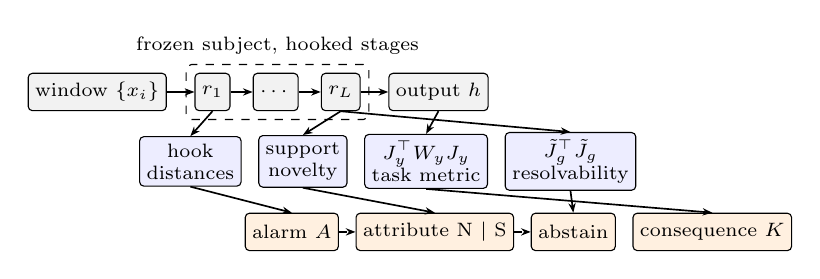
\begin{tikzpicture}[
  font=\scriptsize, node distance=3pt,
  b/.style={draw, rounded corners=1.5pt, inner sep=2.5pt, minimum height=1.35em, align=center},
  sub/.style={b, fill=gray!10}, mon/.style={b, fill=blue!7}, dec/.style={b, fill=orange!12},
  arr/.style={-{Stealth[length=3.5pt]}, semithick}]
  \node[sub] (x) {window $\{x_i\}$};
  \node[sub, right=10pt of x] (r1) {$r_1$};
  \node[sub, right=8pt of r1] (r2) {$\cdots$};
  \node[sub, right=8pt of r2] (rL) {$r_L$};
  \node[sub, right=10pt of rL] (h) {output $h$};
  \draw[arr] (x)--(r1); \draw[arr] (r1)--(r2); \draw[arr] (r2)--(rL); \draw[arr] (rL)--(h);
  \node[draw, dashed, rounded corners=2pt, inner sep=3pt, fit=(r1)(rL), label={[font=\scriptsize]above:frozen subject, hooked stages}] (frz) {};
  \node[mon, below=9pt of r1, xshift=-8pt] (a) {hook\\ distances};
  \node[mon, right=6pt of a] (v) {support\\ novelty};
  \node[mon, right=6pt of v] (pb) {$J_y^{\top}W_yJ_y$\\ task metric};
  \node[mon, right=6pt of pb] (fr) {$\tilde J_g^{\top}\tilde J_g$\\ resolvability};
  \draw[arr] (r1.south) -- (a.north); \draw[arr] (rL.south) -- (v.north);
  \draw[arr] (h.south) -- (pb.north); \draw[arr] (rL.south) -- (fr.north);
  \node[dec, below=9pt of v, xshift=-4pt] (alarm) {alarm $A$};
  \node[dec, right=6pt of alarm] (attr) {attribute N $\mid$ S};
  \node[dec, right=6pt of attr] (abst) {abstain};
  \node[dec, right=6pt of abst] (K) {consequence $K$};
  \draw[arr] (a.south) -- (alarm.north); \draw[arr] (v.south) -- (attr.north);
  \draw[arr] (fr.south) -- (abst.north); \draw[arr] (pb.south) -- (K.north);
  \draw[arr, dashed] (alarm.east) -- (attr.west);
  \draw[arr, dashed] (attr.east) -- (abst.west);
\end{tikzpicture}
\vspace{-0.4em}
\caption{Monitor stack on a frozen subject. Hooked stages feed the
intermediate-hook statistics (reference distances of pooled stage means and
second moments, reference principal coordinates); the output map feeds the
task metric $M_{\mathrm{task}}$ and, through the reconstruction, the
measurement metric $M_{\mathrm{recon}}$. Alarm, N/S attribution, abstention
and the harm measure $K$ are separate endpoints; abstention is a support
novelty with a clean-window conformal threshold.}
\label{fig:stack}
\vspace{-0.6em}
\end{figure}

\section{Two claims}
\label{sec:claims}

The study makes exactly two primary scientific claims, each with one
predeclared paired estimand. Everything else in this note --- detection power,
monitoring cost, physical-variable probes, the designed perturbation
controls, resolvability and patching analyses --- is a supporting analysis or
a positive control, reported where useful and never numbered as a claim.

\textbf{Claim 1 --- incremental attribution value.} On declared,
alarm-time-observable interventions, do intermediate representations improve
acquisition-versus-valid-physics attribution beyond a strong generic monitor
that already receives every operational input-quality, output, uncertainty,
final-embedding and noise-only feature \emph{and the same reference-distance
transforms}? The estimand is the paired difference on a frozen \emph{hard}
evaluation set of N and S windows with overlapping generic signatures,
\[
\Delta\mathrm{F1}_{\mathrm{attr}}=\mathrm{F1}(\texttt{full\_intermediate})-\mathrm{F1}(\texttt{generic\_rich}),
\]
macro-F1 over $\{$N,S$\}$,
where \texttt{generic\_rich} is the committed generic arm and
\texttt{full\_intermediate} adds only information genuinely absent from it:
statistics of strictly internal hooks, with no whitened-input, final-embedding,
pre-output or output duplicate. Controls: a generic arm with matched feature
count (a quadratic expansion of its own scalars), hook-drop arms, and the
internal hooks alone. Provisional reading, unfrozen until justified against
achievable precision: benefit needs a 95\% interval above zero and a point
estimate of at least $0.10$; equivalence needs the whole interval inside
$\pm0.05$; a set below a declared minimum size yields no reading. Required
supporting results: inclusive and hard-matched results with retained
fractions; confusion matrices; family and held-out-severity results;
noise-only and capacity ablations; operational versus privileged variants;
selective risk and retained coverage under abstention; and a joint operational
table over clean, N, S, mixture and unknown windows, so that a good
conditional N/S classifier is not mistaken for a deployed decision rule.
\emph{Refutation:} equivalence or detriment on the hard contrasts, or a gain
attributable to extra input/output transformations, noise-only records,
feature count, event identity or unavailable side information.

\textbf{Claim 2 --- incremental harm ranking.} Does a predeclared
task-sensitive representation score rank scientific harm better than the
committed generic score on held-out, physically generated intervention
cells? With $K$ an independent physical endpoint (amplitude error against
evaluation-only truth on the waveform tier; angular error on a
neutrino-telescope subject), harm $K\ge\kappa_m$, and both scores fixed
without evaluation labels,
\[
\Delta\mathrm{AUROC}_{\mathrm{harm}}=A_{K\ge\kappa_m}(\text{task})-A_{K\ge\kappa_m}(\text{generic}),
\]
with $A_{K\ge\kappa_m}(\cdot)$ the AUROC of a score for harm over all
held-out cells under a frozen cell weighting. The generic score is
committed in advance as the maximum of clean-calibrated reference distances of
the whitened input, the outputs and the final embedding; the task-sensitive
score is the clean-calibrated task length of Section~\ref{sec:mechanism}.
Selecting the better of several generic scores after evaluation is
prohibited. The interval resamples the unit the claim generalizes over ---
the intervention cell --- with event groups nested inside and model seeds as
declared; with too few cells the interval is reported as descriptive and no
confirmatory inference is made. Required supporting results: both absolute
AUROCs, AUPRC with prevalence, the four alarm--harm quadrants with counts at a
cell-level threshold calibrated on clean windows, the missed-harm rate at the
alert budget, false rejection of benign valid-rare cells, family and severity
breakdowns; the conditional strong-alarm triage is secondary and reports how
many cells the conditioning dropped. $\kappa_m$ must be declared from a
scientific requirement before evaluation; it is \emph{pending} on every arm,
development runs use a provisional 10\% amplitude degradation and say so, and
the confirmatory runner refuses while any $\kappa_m$ is pending or any
freeze, environment, data or model hash is missing. \emph{Refutation:} a
paired interval including zero without meeting a predeclared equivalence
rule, systematic low-alarm/high-harm failures, or a gain that disappears on
held-out physical families.

\begin{center}
\scriptsize
\captionof{table}{Claim 2: alarm--harm quadrants and endpoints (cell level).}
\begin{tabularx}{\columnwidth}{@{}p{0.62in}YY@{}}
\toprule
\mbox{} & $K<\kappa_m$ & $K\geq\kappa_m$ \\
\midrule
Low alarm & quiet/benign & missed harm \\
Strong alarm & harmless alarm & detected harm \\
\midrule
\multicolumn{3}{@{}p{\columnwidth}@{}}{\textbf{Primary:} paired
$\Delta\mathrm{AUROC}_{\mathrm{harm}}$ over all held-out cells, cell-outer
resampling. \textbf{Supporting:} absolute AUROCs; AUPRC with prevalence;
missed-harm rate at the budget; benign valid-rare cell rejection (and the
window-level estimator); breakdowns; conditional strong-alarm triage with the
number of cells dropped. All four quadrants are reported with counts.} \\
\bottomrule
\end{tabularx}
\label{tab:c4}
\vspace{-0.3em}
\end{center}

\textbf{Supporting analyses.} \emph{Detection}: power at a 1\% false-alert
rate on non-overlapping clean windows and delay in windows, with a binomial
interval on the realized rate --- a hundred clean windows resolve 1\% in
one-percent steps only, so calibration counts are an output of a development
precision study. \emph{Cost}: latency and storage of sampling and sketching
against full capture, measured on a named machine. \emph{Probes}: ridge
probes from hooked representations to the tier's physical variables, reported
descriptively; probe accuracy is never read as a physical axis.
\emph{Designed controls}: output-null, output-aligned, random and
task-specific aligned/null families, constructed from the frozen head and
therefore positive controls for any monitor built from that head; exact only
for the tied linear subject, refused for nonlinear subjects until a
constrained local inverse with an input-validity check exists; norm matched in
the alarm metric being challenged; realized physical loss reported per
output, with the local-linear error. \emph{Resolvability and patching}: the
rank of $M_{\mathrm{recon}}$ and activation patching are mechanistic
diagnostics; uniform recovery at every stage, which the linear subject
shows, is not localization.

\textbf{Abstention.} Abstention is a feature-novelty rule: the support score
of Section~\ref{sec:mechanism} with a threshold set by split-conformal
calibration on clean calibration windows~\cite{angelopoulos2021}. Under
exchangeability of those windows with deployment \emph{clean} windows the
retained fraction of clean windows is at least $1-\alpha$ in expectation; the
rule guarantees nothing about arbitrary unknown families, so unknown-family
detection is measured empirically (AUROC), together with the risk--coverage
curve and its area, retained coverage at the threshold, and retained-known
macro-F1 with counts~\cite{geifman2017}. Unknown families appear only in the
evaluation partition. Retained coverage is a reporting point, not a threshold
tuned on confirmatory labels.

\textbf{Identifiability and origin.} All attribution is over declared
intervention families under a stated simulator; observing a response profile
does not identify the cause of an unknown real shift, and such windows are
routed to abstention. Origin (N, S, geometry, mixture, unknown) and harm
(benign, harmful) are scored as separate axes: a clean rare event can be
harmful and a mild corruption benign.

\section{Testbeds and monitoring design}
\label{sec:testbeds}

The three tiers are three physically different measurement systems ---
cryogenic-style waveforms with a calibrated covariance, neutrino-telescope
point clouds with no covariance at all, and a SQUID time series with recorded
truth --- under one principle. Generality is claimed across measurement
regimes, not across architectures.

\textbf{Tier 2 --- neutrino-telescope point clouds (realism:
ORACLE-Paired).} One primary public configuration with a released checkpoint.
The intermediate arm hooks all four DynEdge convolution blocks plus the
post-processing and readout stages, not only the 128-dimensional pre-head
event representation. The data are our own production: the released NuBench
datasets are independent per-geometry productions and share no latent events,
so the paired detector-geometry contrast is constructed by re-simulation ---
Prometheus~\cite{prometheus} re-uses one seeded injection across detector
geometries (here ORCA and ARCA, both water, so layout is not confounded with
medium and the photon stage is exactly reproducible), with the NuBench
detector-response emulation reimplemented in-project, which is precisely where
the acquisition knobs live. Per geometry, from one injection: module dropout,
hit thinning, time jitter, gain drift and noise-rate cells instantiate N; S
windows use clean low-density strata in energy, topology, vertex/containment,
and multiplicity, estimated from training data only --- with the caveat that
module loss \emph{lowers} observed multiplicity, so every N cell is matched
by clean events at the same observed multiplicity, charge, and time spread;
otherwise attribution reduces to recognizing the corruption operator's
fingerprint. Undeclared families (double-bang $\nu_\tau$, through-going
muons, pile-up, correlated module noise) are held entirely outside the
declared contract for the abstention endpoint, and the injection identifier is
the pairing key across geometries. One secondary architecture serves as a
consistency check. Until the paired set exists, the released Hexagon water/ice
pair supports only a distribution-level medium comparison, and is labelled as
such. No assumed covariance exists in this tier --- deliberately: it tests,
out of sample, the monitor-failure predictions pre-registered on Tier 1, and
it is where the one alarm computable \emph{without} knowing $\Sigma$ (the
task length in $M_{\mathrm{task}}$, which needs only $J_y$) earns its
deployability claim.

\textbf{Tier 1 --- controlled waveforms (mechanism: ORACLE-Cov).} The
synthetic arm uses a noise-aware linear control and a generator that
constructs PSD/cross-spectral density models, samples seeded frequency-domain
coefficients with real-signal symmetry, and adds declared artifacts; the
generator reports both the implied and the realized covariance of every
ensemble. The synthesis itself is not claimed as novel: \texttt{pytessim} draws
from a cross-spectral density by per-frequency Cholesky
factorisation~\cite{pytessim}, and Wire-Cell colours per frequency band with
user-supplied matrices $A$ satisfying $AA^{\top}\approx\Sigma$~\cite{wirecell}.
Reporting the \emph{realized} covariance of the drawn ensemble, so that
$\hat\Sigma\neq\Sigma$ is measured rather than nominal, is what neither does and
what this tier requires. The inverse-PSD-weighted training objective makes the encoder's
assumed covariance $\hat\Sigma$ a literal property of the loss, so
$\hat\Sigma\neq\Sigma$ is a controlled experimental lever, swept through
the condition number $\kappa(\hat\Sigma^{-1}\Sigma)$. Every theoretical
claim is decided here, and the power analysis that sizes the other tiers runs
here, because only here is the null exactly simulable. Development runs on an
analytic linear subject (September 2026; not results of the study) shape the
arms above: noise-only statistics alone separate covariance-type acquisition
changes from physics changes, covariance mismatches of condition number
5--12 produce large alarms with little consequence on that subject, in-span
rare physics raises the consequence while leaving every noise-only statistic at
its reference, structural acquisition changes move the representation with
out-of-span fractions near one, and activation patching is flat --- so stage
localization is a question for the nonlinear subject, and any attribution
gain of an intermediate arm must be shown to exceed what the generic arm with
noise-only records and the same distance transforms already gives. A first
development smoke of the two-claim protocol on the linear subject (16
September 2026; non-citable, toy size) found no reading on its 20-window hard
set, a small inclusive gain that a capacity-matched generic arm largely
absorbed, and a Claim-2 difference whose cell-outer interval included zero.

\textbf{Tier 3 --- TIDMAD (real data).} The public TIDMAD~\cite{tidmad} arm
uses a $\sim0.6$M-parameter two-stage domain transformer, comparing otherwise
identical MSE and inverse-PSD-weighted objectives --- two assumed covariances
on identical real electronics noise, the naturally occurring real-data echo of
the Tier-1 contrast. The release's denoising score is a development
consequence only; the confirmatory consequence is the relative
exclusion-limit comparison. This compact transformer is a diagnostic subject,
not a foundation model; a larger pretrained model is only a later gated
comparison.

\textbf{Monitoring comparison.} Every arm consumes only features available at
alarm time, built through a typed input object that carries the observed
window, its random-trigger records and the geometry --- and nothing else ---
so that truth, the paired replay, the realized covariance and the intervention
label are not arguments of any alarm-time builder; every feature carries its
source tags and an arm is scored only from a locked, tag-checked batch. (A
builder that lies about a tag is not caught; code review remains part of the
contract.) One regularized logistic classifier, one tuning grid and one set
of partitions serve every arm. Partitions are five, split by event group so
that every geometry, replay and corruption variant of an event stays
together: reference fitting (clean subject, projectors, nulls --- never
supervised examples), attribution training, development (tuning), clean
calibration (false-alert budget, conformal threshold) and evaluation, scored
once. Held-out families, severities and seeds are declared and scored on
evaluation groups only; undeclared families enter no fit, tuning or
calibration. The primary arms are \texttt{generic\_rich} (input quality,
outputs, an uncertainty proxy, the final embedding, operational noise-only
statistics, and reference distances of the whitened input, the outputs, the
pre-output, the energy split of the final embedding, the out-of-span fraction
and the support novelty), \texttt{intermediate\_only} (reference distances of
the pooled mean and second moment of each internal hook and its reference
principal coordinates) and \texttt{full\_intermediate}; controls are a
capacity-matched generic arm and hook-drop arms. Noise-only statistics are
operational only where the acquisition supplies random-trigger records (the
controlled simulator, the HeST arm and TIDMAD's no-injection files do;
hit-level Prometheus output does not, and such an arm is reported as
privileged). Reference distances use Ledoit--Wolf shrinkage~\cite{ledoitwolf2004} and, where a hook's
dimension exceeds a fifth of the reference count, a reference-fitted PCA; each
is mapped to a common clean-null scale before any combination, and their
stability across reference sample size and rescaling is tested --- at the
reference sizes of a development smoke they are not stable, which the report
states. Hard contrasts are built by 1:1 matching of S to N windows inside a
declared caliper on standardized generic signatures, with retained fractions
and overlap failures reported; matching is a declared conditional design, not
a causal identification. Eligible baselines --- corrected univariate input
tests, RBF-MMD~\cite{gretton2012}, a classifier two-sample
test~\cite{lopezpaz2017}, embedding mean/covariance distance, output tests,
uncertainty/entropy --- receive identical windows and false-alert budgets.
Clean miscalibration is a model result, not automatically a software
bug~\cite{guo2017}. Intervals resample event groups for window-level
estimands and intervention cells for cell-level ones, with model seeds as a
declared level; null results require a passed positive control, adequate
precision and a predeclared equivalence margin.

\textbf{Reporting standard.} Every learned arm and baseline is reported with
its parameter count, training cost, and inference time and memory per event,
and arms compared against each other are matched in parameter count, not in
tuning effort. Every endpoint is reported inclusively and on the stratum where
the methods are predicted to differ (highest severity, lowest SNR, boundary
support), under the same metric names on every tier. Every threshold ---
alarm, attribution, abstention --- is reported as a curve at the
pre-registered false-alert budget (risk--coverage for abstention), never as a
single operating point. Each learned ladder contains an extrapolation arm
trained inside and evaluated outside the declared severity and multiplicity
range, labelled as such. The hyperparameters of every method appear in one
table with the values used.

\begin{figure*}[!t]
  \centering
  \begin{minipage}[b]{0.43\textwidth}
    \centering
    \includegraphics[width=\linewidth,height=0.88in,keepaspectratio]{figures/nubench_detector_geometries.png}\\[-0.2em]
    \scriptsize (a) detector geometries
  \end{minipage}\hfill
  \begin{minipage}[b]{0.25\textwidth}
    \centering
    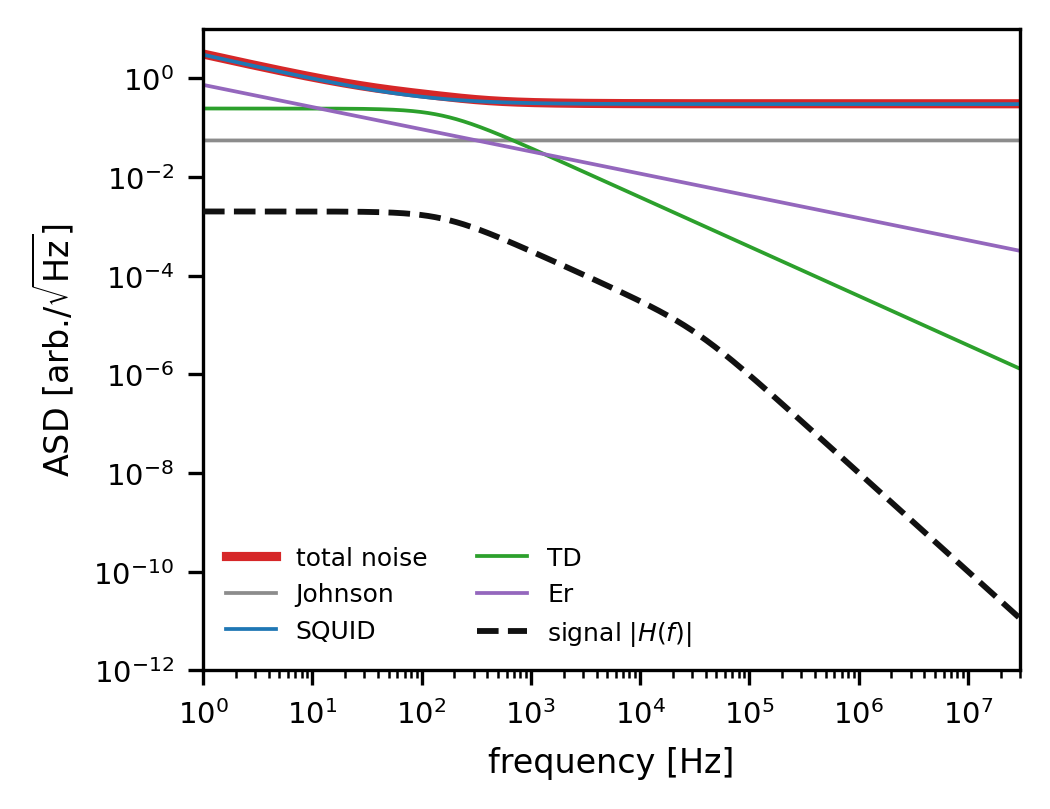
\includegraphics[width=\linewidth,height=0.88in,keepaspectratio]{figures/spectrum_detector_signal_noise.png}\\[-0.2em]
    \scriptsize (b) detector signal/noise spectrum
  \end{minipage}\hfill
  \begin{minipage}[b]{0.28\textwidth}
    \centering
    \includegraphics[width=\linewidth,height=0.88in,keepaspectratio]{figures/noise_generator_examples.png}\\[-0.2em]
    \scriptsize (c) generated waveform stress tests
  \end{minipage}
  \vspace{-0.45em}
  \caption{Complementary testbeds. (a) Six top-view geometries, reproduced
  from NuBench Fig.~3~\cite{nubench}. (b) The analytic Al$_2$O$_3$/Al
  athermal reference budget --- component and total noise ASDs with the
  two-pole signal response --- regenerated from the parameterised model in
  \texttt{noise\_module.reference\_budget}. (c) The generator composes a
  clean optimal-filter-like pulse with stationary colored noise, piecewise
  nonstationarity, and explicit artifacts. Panels (b)--(c) are project
  outputs.}
  \label{fig:testbeds}
  \vspace{-0.7em}
\end{figure*}

\begin{center}
\scriptsize
\captionof{table}{Experiment matrix. The two claims run on the trained
Tier-1 subject and one transfer arm; the rest are supporting analyses.}
\begin{tabularx}{\columnwidth}{@{}p{0.16in}p{0.95in}Y@{}}
\toprule
ID & Test & Endpoints \\
\midrule
E0 & Clean replay; deliberate evaluation-contract faults (EF) & Reference
discrepancy; gate sensitivity/specificity (gate, not a claim) \\
A1 & Claim 1: hard-matched N/S attribution, primary arms and controls,
abstention, joint decision table & $\Delta\mathrm{F1}_{\mathrm{attr}}$ with
interval; ablations; unknown AUROC; risk--coverage; joint table \\
A2 & Claim 2: harm ranking on held-out cells & $\Delta\mathrm{AUROC}_{\mathrm{harm}}$
with cell-outer interval; quadrants; missed harm; valid-rare rejection \\
S1 & Detection power and delay at 1\% FAR & power, delay, realized FAR with
binomial interval (supporting) \\
S2 & Designed and task-specific controls & realized per-output loss at matched
norm; local-linear error (positive control) \\
S3 & Probes, resolvability, patching & probe $R^2$; rank of
$M_{\mathrm{recon}}$; patched-$K$ recovery (mechanistic, descriptive) \\
S4 & Capture vs sample/sketch & p50/p95 latency; bytes/event; loss (supporting) \\
T1 & Transfer: the two claims repeated once on one held-out physical arm &
same estimands, predeclared; failures reported as failures \\
\bottomrule
\end{tabularx}
\label{tab:experiments}
\vspace{-0.5em}
\end{center}

\section{Evidence ladder and roadmap}

\begin{tcolorbox}[colback=black!3,colframe=black!35,boxrule=0.4pt,
  left=4pt,right=4pt,top=3pt,bottom=3pt,arc=1pt]
\footnotesize
\textbf{Minimum viable paper.} (1)~The two claims on the controlled waveform
tier with a \emph{trained nonlinear} subject; (2)~the two claims repeated once
on one independent transfer arm chosen by readiness, licence and physical-$K$
gates (HeST $\to$ our readout is built; LUCiD is licence-gated; Prometheus is
the fallback with a frozen public model and angular error as $K$); (3)~the
paired comparisons with their failures and limitations. TIDMAD is an external
check if its relative exclusion-limit endpoint survives scrutiny.

\textbf{Phase A --- theory and schema gate (this revision).} Two metrics
separated; resolvability renamed; support estimated; conditional signatures;
invariance controls; protocol layer hardened; development smoke. No trained
campaign starts before adversarial review of this phase.

\textbf{Phase B --- precision and feasibility (development only).}
Calibration size for the false-alert budget; outer-unit counts for Claim~2;
model-seed variability; matched-contrast overlap. Unachievable precision
changes the claim or the design before any freeze.

\textbf{Phase C --- scientific evidence.} The trained Tier-1 subject in
development mode; if controls and hard contrasts pass, exactly one transfer
arm; freeze only after thresholds, hold-outs, cell weights, scores, margins,
counts and dependency hashes are agreed.

\textbf{Future work, not this paper.} Additional geometries, the linear
estimator classes as probes of physical axes, sampling-cost optimization,
Panda/SPINE transfer, and stage localization, unless one of them directly
resolves a claim.
\end{tcolorbox}

\textbf{Relation to chained-model uncertainty propagation.} Douglas et
al.~\cite{douglas2024} propagate input uncertainty through a chained
neutrino-LAr reconstruction and compare uncertainty-aware and blinded models
under synthetic noise. Here the model is frozen: the question is whether its
representation attributes a declared failure, abstains outside scope, and
links an alarm to consequence. Propagated uncertainty is therefore a candidate
covariate, not the endpoint.

\textbf{Relation to shift monitoring and localization.} The components of this
study are individually established, and we claim the physics instantiation and
the evaluation protocol, not the components. Shift-type identification from a
frozen encoder exists in medical imaging~\cite{roschewitz2024}, building on
the acquisition-versus-population taxonomy of~\cite{castro2020}; harmful-%
versus-benign shift detection is a named research line~\cite{podkopaev2022,
rabanser2019}, and performance changes have been attributed to specific shift
mechanisms~\cite{zhang2023}. That shift type determines \emph{which layers} to
adapt is the headline of surgical fine-tuning~\cite{lee2023surgical}, and
localization-then-edit validation is known to be a weak inference~%
\cite{hase2023}, which is why any later repair experiment here is preceded by
an activation-patching causal check rather than resting on adaptation gains.
Unlabelled performance estimation~\cite{guillory2021,garg2022} predicts a
classifier's aggregate accuracy on a shifted distribution from confidences,
under assumptions on the shift that its authors state cannot be verified from
unlabelled data alone. What none of these supply, and what this study tests,
is (i) a consequence variable that is a physics observable under a known
measurement covariance rather than classification accuracy, (ii) the paired
all-cell alarm--harm comparison of Table~\ref{tab:c4}, including harm that
arrives without a strong alarm, with designed dissociations as positive
controls, and (iii) an attribution comparison whose generic arm already
holds the acquisition's own noise-only statistics and the same distance
transforms as the intermediate arm. We are not
aware of a monitoring result for learned neutrino-telescope reconstruction and
do not claim the absence of one.

\section{Collaboration}

The agreed sequence is B$\rightarrow$A$\rightarrow$A$\oplus$B, while the
waveform/TIDMAD arm runs in parallel and supplies the first code-complete
contrast. Work is consolidated in the shared ORACLE repository. A proposed
fortnightly meeting reviews one frozen
protocol or result; initial ownership is waveform infrastructure and generic
monitoring on Dowling's side, and geometry/SPINE physics choices and validation
on Junjie's side, with thresholds and claim changes approved jointly. The first
meeting should freeze one geometry intervention, pairing variables, one
representation endpoint, and one downstream physics endpoint.

\section{Feasibility gate}

Dataset access, checkpoint loading, released-prediction rescoring,
intermediate-hook extraction, and a monotone module-dropout positive control
have been validated ($15.28^\circ\!\to\!25.12^\circ$ median angular error and
10-NN retention $1.000\!\to\!0.393$ across $0$--$50\%$ dropout), with the
caveat that the pilot sample was enriched and non-randomly drawn; the audited
scripts redraw it uniformly with nested severities and paired intervals.
Exact re-inference parity remains unresolved: the current pipeline differs
from the released directions by $0.944^\circ$ median angular error. Two
identified confounds are resolved first: the released-metric rescoring had
grouped by the track/cascade topology flag while Table~6 categories are
interaction classes, and the pilot substitutes five preprocessing methods of
the released detector, which is itself a candidate cause and is now disclosed
with the outputs. The decisive next test is cheap: identical re-inference on
CPU and GPU separates a $k$-NN backend cause (CPU$\neq$GPU) from
preprocessing, alignment, or version skew (CPU$=$GPU$\neq$release). Exact
identity is a software control, separate from the scientific geometry gate. On
a fixed development subset we will test whether the residual offset is stable
across severity and event strata. Stable offsets permit a predeclared backend
tolerance for the paired contrast; severity-dependent drift is a confound and
keeps the gate closed.

\begin{thebibliography}{99}
\scriptsize
\setlength{\itemsep}{-1.6pt}\setlength{\parsep}{0pt}
\bibitem{nubench} R.~F. \O rs\o e et al. ``NuBench: An Open Benchmark for Deep
Learning-Based Event Reconstruction in Neutrino Telescopes.'' JINST 21 (2026).
\href{https://arxiv.org/abs/2511.13111}{arXiv:2511.13111}.
\bibitem{koh2020} D.~H. Koh et al. (DeepLearnPhysics). ``Scalable,
Proposal-free Instance Segmentation Network for 3D Pixel Clustering and
Particle Trajectory Reconstruction in LArTPCs.''
\href{https://arxiv.org/abs/2007.03083}{arXiv:2007.03083} (2020).
\bibitem{douglas2024} D. Douglas, A. Mishra, F. Petersen, D. Ratner,
K. Terao. ``Uncertainty Propagation within Chained Models for Machine Learning
Reconstruction of Neutrino-LAr Interactions.''
\href{https://arxiv.org/abs/2411.09864}{arXiv:2411.09864v3}, preprint (2025).
\bibitem{angelopoulos2021} A.~N. Angelopoulos and S. Bates. ``A Gentle
Introduction to Conformal Prediction.''
\href{https://arxiv.org/abs/2107.07511}{arXiv:2107.07511} (2021).
\bibitem{geifman2017} Y. Geifman and R. El-Yaniv. ``Selective Classification
for Deep Neural Networks.'' NeurIPS (2017).
\bibitem{gretton2012} A. Gretton et al. ``A Kernel Two-Sample Test.'' JMLR 13
(2012), 723--773.
\bibitem{lopezpaz2017} D. Lopez-Paz and M. Oquab. ``Revisiting Classifier
Two-Sample Tests.'' ICLR (2017).
\bibitem{guo2017} C. Guo et al. ``On Calibration of Modern Neural Networks.''
ICML (2017).
\bibitem{roschewitz2024} M. Roschewitz, R. Mehta, C. Jones, B. Glocker.
``Automatic Dataset Shift Identification to Support Safe Deployment of Medical
Imaging AI.'' MICCAI (2025).
\href{https://arxiv.org/abs/2411.07940}{arXiv:2411.07940}.
\bibitem{castro2020} D.~C. Castro, I. Walker, B. Glocker. ``Causality Matters
in Medical Imaging.'' Nature Communications 11, 3673 (2020).
\bibitem{podkopaev2022} A. Podkopaev, A. Ramdas. ``Tracking the Risk of a
Deployed Model and Detecting Harmful Distribution Shifts.'' ICLR (2022).
\href{https://arxiv.org/abs/2110.06177}{arXiv:2110.06177}.
\bibitem{rabanser2019} S. Rabanser, S. G\"unnemann, Z. Lipton. ``Failing
Loudly: An Empirical Study of Methods for Detecting Dataset Shift.'' NeurIPS
(2019).
\bibitem{guillory2021} D. Guillory, V. Shankar, S. Ebrahimi, T. Darrell,
L. Schmidt. ``Predicting with Confidence on Unseen Distributions.'' ICCV
(2021). \href{https://arxiv.org/abs/2107.03315}{arXiv:2107.03315}.
\bibitem{garg2022} S. Garg, S. Balakrishnan, Z.~C. Lipton, B. Neyshabur,
H. Sedghi. ``Leveraging Unlabeled Data to Predict Out-of-Distribution
Performance.'' ICLR (2022).
\href{https://arxiv.org/abs/2201.04234}{arXiv:2201.04234}.
\bibitem{zhang2023} H. Zhang, H. Singh, M. Ghassemi, S. Joshi. ```Why Did the
Model Fail?': Attributing Model Performance Changes to Distribution Shifts.''
ICML (2023). \href{https://arxiv.org/abs/2210.10769}{arXiv:2210.10769}.
\bibitem{lee2023surgical} Y. Lee, A.~S. Chen, F. Tajwar, A. Kumar, H. Yao,
P. Liang, C. Finn. ``Surgical Fine-Tuning Improves Adaptation to Distribution
Shifts.'' ICLR (2023).
\href{https://arxiv.org/abs/2210.11466}{arXiv:2210.11466}.
\bibitem{hase2023} P. Hase, M. Bansal, B. Kim, A. Ghandeharioun. ``Does
Localization Inform Editing? Surprising Differences in Causality-Based
Localization vs.\ Knowledge Editing in Language Models.'' NeurIPS (2023).
\href{https://arxiv.org/abs/2301.04213}{arXiv:2301.04213}.
\bibitem{prometheus} J. Lazar, S. Meighen-Berger, C. Haack, D. Kim,
S. Giner, C.~A. Arg\"uelles. ``Prometheus: An Open-Source Neutrino Telescope
Simulation.'' Comput.\ Phys.\ Commun.\ (2024).
\href{https://arxiv.org/abs/2304.14526}{arXiv:2304.14526}.
\bibitem{kay1993} S.~M. Kay. \emph{Fundamentals of Statistical Signal
Processing: Estimation Theory.} Prentice Hall (1993), ch.~3 (the Cram\'er--Rao
bound and Fisher information for the Gaussian model).
\bibitem{ledoitwolf2004} O. Ledoit and M. Wolf. ``A well-conditioned estimator
for large-dimensional covariance matrices.'' J. Multivariate Anal. 88 (2004),
365--411.
\bibitem{paper1} D. Wong. ``Noise Covariance Defines Reconstruction
Geometry: Optimal Filtering, Weighted Subspaces, and Tied Linear
Autoencoders.'' Preprint (2026), unpublished at the time of writing; cited for
the covariance-weighted linear classes only, no central result of this note
depends on it.
\bibitem{pytessim} TESSERACT Collaboration. ``\texttt{pytessim}: simulation of
TES datastreams including noise, LEE, and signals.'' MIT-licensed software,
first public release 2026-05-18.
\href{https://github.com/spice-herald/pytessim}{github.com/spice-herald/pytessim}.
Multichannel noise sampled from a PSD or cross-spectral density by
per-frequency Cholesky factorisation (\texttt{core/noise/Noise\_Factory.py}).
\bibitem{wirecell} Wire-Cell Team. ``Wire-Cell Toolkit.'' LGPL-licensed
software. \href{https://github.com/WireCell/wire-cell-toolkit}{github.com/WireCell/wire-cell-toolkit}.
\texttt{gen/src/CorrelatedAddNoise.cxx} (added 2026-02-04) colours per frequency
band with user-supplied matrices $A$ satisfying $AA^{\top}\approx$ the
correlation matrix; \texttt{CoherentAddNoise} with \texttt{GroupNoiseModel}
gives shared-private block structure.
\bibitem{microboone2017noise} MicroBooNE Collaboration. ``Noise
Characterization and Filtering in the MicroBooNE Liquid Argon TPC.''
JINST 12, P08003 (2017).
\href{https://arxiv.org/abs/1705.07341}{arXiv:1705.07341}.
\bibitem{panda2} S. Young, C. Jes\'us-Valls, K. Terao. ``Panda Diplomacy:
Foundation Model Pre-training across Particle Imaging Detectors for High
Energy and Nuclear Physics.''
\href{https://arxiv.org/abs/2609.00611}{arXiv:2609.00611} (2026).
\bibitem{gravnet} S.~R. Qasim, J. Kieseler, Y. Iiyama, M. Pierini.
``Learning representations of irregular particle-detector geometry with
distance-weighted graph networks.'' Eur.\ Phys.\ J.\ C 79, 608 (2019).
\href{https://arxiv.org/abs/1902.07987}{arXiv:1902.07987}.
\bibitem{objcond} J. Kieseler. ``Object condensation: one-stage grid-free
multi-object reconstruction in physics detectors, graph and image data.''
Eur.\ Phys.\ J.\ C 80, 886 (2020).
\href{https://arxiv.org/abs/2002.03605}{arXiv:2002.03605}.
\bibitem{fmbench} M. Chu, Y. Liu, A. Biswas, H.-W. Shen. ``Do Physics Foundation Models Learn Generalizable Physics?
A Bias-Aware Benchmark Across Physical Regimes and Distribution Shifts.''
\href{https://arxiv.org/abs/2605.29283}{arXiv:2605.29283} (2026).
\bibitem{tidmad} J. Fry, X. Fu, Z. Fu, K. Pappas, L. Winslow, A. Li.
``TIDMAD: Time-Series Dataset for Discovering Dark Matter with AI Denoising.''
NeurIPS Datasets \& Benchmarks (2025).
\href{https://arxiv.org/abs/2406.04378}{arXiv:2406.04378}.
\end{thebibliography}

\end{document}
